\documentclass{article}
% Language setting
%\addbibresource{sample.bib}
\usepackage[english]{babel}
\usepackage{xcolor}
\usepackage{soul}
% Set page size and margins
% Replace `letterpaper' with `a4paper' for UK/EU standard size
\usepackage[letterpaper,top=2cm,bottom=2cm,left=3cm,right=3cm,marginparwidth=1.75cm]{geometry}

% Useful packages
\usepackage[colorlinks=true, allcolors=blue]{hyperref}
\usepackage{amsmath}
\usepackage{graphicx}
\usepackage{amssymb}
\usepackage{hyperref}
\usepackage{tikz}
\usepackage{booktabs}
\usepackage{pgfplots}
\usepackage{indentfirst}
\usepackage{subcaption}
\usepackage{algorithm} 
\usepackage{algpseudocode}
\usepackage{pgfplots}
\usepackage{pgfplotstable}
\usetikzlibrary[quotes, calc, arrows.meta, plotmarks]
% \usetikzlibrary{external}
% \tikzexternalize[prefix=tikz/]
%\usepgfplotslibrary{external}
%\tikzexternalize

\makeatletter
\renewcommand*\env@matrix[1][\arraystretch]{%
  \edef\arraystretch{#1}%
  \hskip -\arraycolsep
  \let\@ifnextchar\new@ifnextchar
  \array{*\c@MaxMatrixCols c}}
\makeatother

\providecommand{\keywords}[1]
{
  \small	
  \textbf{\textit{Keywords---}} #1
}

\pgfplotsset{compat = newest}

\title{A Flow-Structure Interaction Method...}

\author{Daniel B. V. Santos$^*$$^a$ \\
email:\href{daniel.barbedo@coppe.ufrj.br}{daniel.barbedo@coppe.ufrj.br}
\and
Gustavo R. Anjos$^a$ \\ email:\href{gustavo.rabello@coppe.ufrj.br}{gustavo.rabello@coppe.ufrj.br}
\and
Marcelo A. Savi$^a$ \\ email:\href{savi@mecanica.coppe.ufrj.br}{savi@mecanica.coppe.ufrj.br}
}
\date{%
\begin{small}
    % $^a$COPPE/Departamento de Engenharia Mecânica - Universidade Federal do Rio de Janeiro, Rua Moniz Aragão Nº 360, Bloco 1, Rio de Janeiro, Brasil.\\%
    $^a$COPPE - Department of Mechanical Engineering, Universidade Federal do Rio de Janeiro (UFRJ)
    Av. Horacio Macedo, 2030, Cidade Universitária,  Rio de Janeiro, Brazil. Zip Code 21945-970 \\%
    $^*$Corresponding Author.\\[2ex]%
    \today
\end{small}
}

\begin{document}
\maketitle

\begin{abstract}

\end{abstract}

\keywords{Fluid-Structure Interaction, Finite Element Method, Van der Pol Oscilator, CFD}

\section{Introduction}

In the interest of accurately representing the fluid induced vibrations on piping, and therefore the available energy to be converted into electric energy to be stored and remotely power smart materials, a flow-structure simulation using the finite element method to represent both the flow and the solid structure was developed.


This work presents a methodology for the numerical simulation of fluid–structure interaction (FSI), along with its verification. The fluid phase is governed by the Navier–Stokes equations, solved using the finite element method on an unstructured mesh, with a first-order semi-Lagrangian scheme employed for the discretization of the nonlinear convective term. The solid phase is modeled through the discretized balance of momentum equation, adopting either a linear elastic model or a Saint-Venant–Kirchhoff constitutive law. While the solid is described in a Lagrangian formulation, the fluid domain is expressed in an Eulerian framework; to consistently account for mesh motion, an Arbitrary Lagrangian–Eulerian (ALE) approach is employed. The numerical implementation is first verified independently for each phase and subsequently for the coupled problem. Finally, several FSI test cases are presented, encompassing a range of material properties and flow conditions.

%Using this numerical tool, several Reynolds numbers were simulated, and the displacements and forces in the solid structure produced by the flow measured. In turn, an oscillator function similar to a van der pol oscillator was used to fit the displacement and force data as a function of the Reynolds number, producing an accurate representation of the flow-structure interaction induced vibrations for a given Reynolds range that is accurate, readily available, and does not require lengthy numerical simulations.

\section{Governing Equations}

The fluid is represented by the incompressible Navier-Stokes equations, ignoring the effect of gravity forces. Their dimensional form is given by:

\begin{equation}
	\nabla \cdot \mathbf{v} = 0
\end{equation}

\begin{equation}	
	\rho \frac{\partial \mathbf{v}}{\partial t}
	+ \mathbf{c} \cdot \nabla \mathbf{v}
	= -\nabla p
	+ \mu \nabla^2 \mathbf{v}
	\label{eq:Momentum}
\end{equation} \\

\noindent where $\mathbf{v}$ represents the velocity, $p$ the pressure and $\rho$ and $\mu$ are the specific mass and viscosity of the fluid, respectively. In order to accomodate the solid displacement, a moving mesh or remeshing strategy is necessary. For this work, we chose to follow the ALE methodology. In order to implement this method, the advection velocity in the material derivative needs to be replaced by the $\mathbf{c}$ velocity, more details can be found in \cite{anjos_moving_2021}. This velocity is given by:

\begin{equation}
	\mathbf{c} = \mathbf{v}_{fluid} - \mathbf{v}_{mesh}
\end{equation} \\

The solid is represented by the dynamic momentum balance equation, with no damping terms, given by:

\begin{equation}
	\nabla \cdot \sigma
	- \rho_s \frac{\partial ^2 \mathbf{u} }{\partial t ^2 } = f
	\label{eq:Solid Momentum}
\end{equation} \\

\noindent where $\sigma$ is the Cauchy stress tensor, $\mathbf{u}$ are the displacements, $\rho_s$ is the specific mass of the solid, and $f$ represents the external forces per unit of area, the traction, acting upon the solid. The Cauchy stress tensor is a function of the strain tensor and the material properties, as follows: 

\begin{equation}
	\sigma = \mathbf{D} \epsilon
\end{equation} \\

In two dimensions, there are only three non-zero components of $\sigma$ and $\epsilon$, which can be written as:

\begin{equation}
	\sigma
	=
	\begin{bmatrix}[2]
		\sigma_{xx} \\
		\sigma_{yy} \\
		\sigma_{xy}
	\end{bmatrix}
	\qquad
	\epsilon
	=
	\begin{bmatrix}[2]
		\epsilon_{xx} \\
		\epsilon_{yy} \\
		\epsilon_{xy}
	\end{bmatrix}
\end{equation} \\

For a two-dimensional plane stress isotropic material $\mathbf{D}$ can be written as:

\begin{equation}
	\mathbf{D}
	=
	\frac{E}{1 - \nu^2}
	\begin{bmatrix}[2.0]
		1	 & \nu	 & 0 \\
		\nu	 & 1	 & 0 \\
		0	 & 0	 & \dfrac{(1-\nu)}{2}
	\end{bmatrix}
\end{equation} \\

\noindent where $E$ is Young modulus and $\nu$ the Poisson coefficient.The strain tensor can be represented as a function of the displacements by:

\begin{equation}
	\epsilon
	=
	\begin{bmatrix}[2.0]
		\dfrac{\partial u}{\partial x} \\
		\dfrac{\partial v}{\partial y} \\
		\dfrac{\partial u}{\partial y} + \dfrac{\partial v}{\partial x} \\
	\end{bmatrix}
	=
	\begin{bmatrix}[2.0]
		\dfrac{\partial}{\partial x} & 0 \\
		0 & \dfrac{\partial v}{\partial y} \\
		\dfrac{\partial}{\partial y} & \dfrac{\partial }{\partial x} \\
	\end{bmatrix}
	\begin{bmatrix}[2.0]
		u \\
		v
	\end{bmatrix}
	=
	\mathbf{L} \mathbf{U}
\end{equation} \\

After multiplying $\mathbf{D}$ and $\epsilon$, $\sigma$ can be expressed as a function of the displacements, as follows:

\begin{equation}
	\sigma
	= \mathbf{D} \mathbf{L} \mathbf{U}
	=
	\begin{bmatrix}[2]
		\dfrac{\partial u}{\partial x}
		+ \nu \dfrac{\partial v}{\partial y} \\		
		\nu \dfrac{\partial u}{\partial x}
		+ \dfrac{\partial v}{\partial y} \\		
		\dfrac{(1-\nu)}{2} \bigg(\dfrac{\partial u}{\partial y}
		+ \dfrac{\partial v}{\partial x} \bigg)	
	\end{bmatrix}
\end{equation} \\

The form given above is one of convenience. The "vector" displayed above is in truth a tensor in the form:

\begin{equation}
	\sigma =
	\begin{bmatrix}[2]
		\sigma_{xx} && \sigma_{xy} \\
		\sigma_{yx} && \sigma_{yy}
	\end{bmatrix}
\end{equation} \\

\noindent where $\sigma_{xy} = \sigma_{yx}$. By taking the divergent of the tensor above, one finds:

\begin{equation}
	\nabla \cdot \sigma =
	\begin{bmatrix}
		\dfrac{E}{1-\nu^2} \dfrac{\partial^2 u}{\partial x^2}
		+ \dfrac{E}{2(1+\nu)} \dfrac{\partial^2 u}{\partial y^2}
		+ \bigg(\dfrac{E \nu}{1-\nu^2} + \dfrac{E}{2(1+\nu)} \bigg) \dfrac{\partial^2 v}{\partial x \partial y} \\
		\dfrac{E}{1-\nu^2} \dfrac{\partial^2 v}{\partial y^2}
		+ \dfrac{E}{2(1+\nu)} \dfrac{\partial^2 v}{\partial x^2}
		+ \bigg(\dfrac{E \nu}{1-\nu^2} + \dfrac{E}{2(1+\nu)} \bigg) \dfrac{\partial^2 u}{\partial x \partial y}		
	\end{bmatrix}	
\end{equation} \\

Replacing the results above in Eq.\ref{eq:Solid Momentum}, and rearranging the terms, the results are given by:

\begin{equation}
	\frac{E}{1 - \nu^2} \left( \frac{\partial^2 u_x}{\partial x^2} + \frac{1 - \nu}{2} \frac{\partial^2 u_x}{\partial y^2} + \frac{\nu + 1}{2} \frac{\partial^2 u_y}{\partial x \partial y} \right)
	- \rho \frac{\partial^2 u_x}{\partial t^2} 
	= f_x
\end{equation}

\begin{equation}
	\frac{E}{1 - \nu^2} \left( \frac{\partial^2 u_y}{\partial y^2} + \frac{1 - \nu}{2} \frac{\partial^2 u_y}{\partial x^2} + \frac{\nu + 1}{2} \frac{\partial^2 u_x}{\partial x \partial y} \right)
	- \rho \frac{\partial^2 u_y}{\partial t^2}
	= f_y
\end{equation} \\

\noindent where $E$ is Young's modulus, $\nu$ is Poisson coefficient, $\rho_s$ is the solid's specific mass, and $f_x$ and $f_y$ are the forces applied in the $x$ and $y$ directions. It is however much more convenient to work with the matricial form of the equation above, which is given by:

\begin{equation}
	\mathbf{L}^T ( \mathbf{D} \mathbf{L} \mathbf{U} ) - \rho_s \frac{\partial ^2 \mathbf{u} }{\partial t ^2 } = \mathbf{f}
	\label{eq:matrix form solid}
\end{equation} \\

\noindent where $\mathbf{L}^T$ represents the operator that returns the divergent of a tensor.
%This equation can also be made non-dimensional using the following terms:
%
%\begin{equation}
%		\mathbf{u}^* = \frac{\mathbf{u}}{L_f}, \quad
%		t^* = \frac{tV_f}{L_f}, \quad
%		\sigma^* = \frac{\sigma}{\rho_f V_f^2}, \quad
%		\rho_s^* = \frac{\mathbf{\rho_s}}{\rho_f}, \quad
%		\nabla^*=\nabla L, \quad		
%		\mathbf{f}^*=\frac{\mathbf{f}}{\rho_f V_f^2}		
%\end{equation} \\
%
%\noindent where $\rho_f$, $L_f$, and $V_f$ represent the fluid specific mass, characteristic velocity, and length, respectively. The non-dimensionalization procedure results on Eq. \ref{eq:matrix form solid} again, but with non-dimensional parameters.

The loads applied to the solid, at the fluid-solid interface, are derived from the newtonion fluid stress tensor, given by:

\begin{equation}
    \mathbf {\tau} = -pI + \mu [ \nabla \mathbf{u} + (\nabla \mathbf{u})^T ]
\end{equation} \\

\noindent where $p$ is the fluid pressure, $I$ is the identity tensor, and $\mu$ is the viscosity of the fluid. The stress tensor is then multiplied by the fluid-solid interface normal, in order to obtain the traction:

\begin{equation}
    t = \mathbf{\tau} \cdot \mathbf{n}
\end{equation} \\

\noindent and the traction can be integrated over the fluid-interface length, in order to obtain the forces applied to the solid.

\section{Numerical Modeling}

Both the Navier-Stokes equations and the dynamic momentum balance of the solid are solved through the finite element method, using the Galerkin discretization. The convective term of the Navier-Stokes equations is non-linear term. This term can generate instability at higher Reynolds numbers when used directly after the Galerkin discretization. In order to avoid this instability, this term is discretized explicitly through a first order semi-Lagrangian method \cite{anjos_one_2022}, which is unconditionally stable.

\begin{figure}
	\centering
	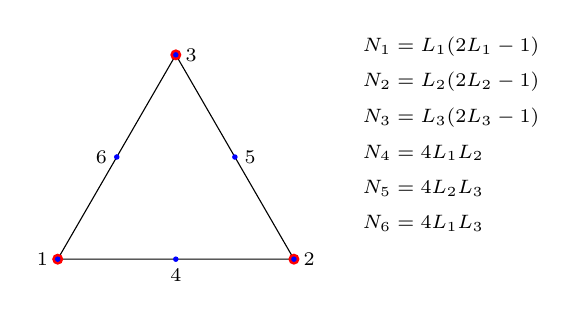
\begin{tikzpicture}[every node/.style={font=\scriptsize}]
		\pgfmathsetmacro\l{3}
		\coordinate (a) at (0, 0);
		\coordinate (b) at (\l, 0);
		\coordinate (c) at (\l/2, \l * 1.73 / 2);		
		\coordinate (d) at (\l/2, 0);
		\coordinate (e) at (\l * 0.75, \l * 1.73 / 4);
		\coordinate (f) at (\l * 0.25, \l * 1.73 / 4);
		\draw[] (a) -- (b) -- (c) -- cycle;
		\fill[red] (a) circle (2pt);
		\fill[red] (b) circle (2pt);
		\fill[red] (c) circle (2pt);
		\fill[blue] (a) circle (1pt);
		\fill[blue] (b) circle (1pt);
		\fill[blue] (c) circle (1pt);
		\fill[blue] (d) circle (1pt);
		\fill[blue] (e) circle (1pt);
		\fill[blue] (f) circle (1pt);
		\node[left] at (a) {1};
		\node[right] at (b) {2};
		\node[right] at (c) {3};
		\node[below] at (d) {4};
		\node[right] at (e) {5};
		\node[left] at (f) {6};		
		\node[right] at (1.25 * \l, 6 * 0.15 * \l) {$N_1 = L_1 (2 L_1 - 1)$};
		\node[right] at (1.25 * \l, 5 * 0.15 * \l) {$N_2 = L_2 (2 L_2 - 1)$};
		\node[right] at (1.25 * \l, 4 * 0.15 * \l) {$N_3 = L_3 (2 L_3 - 1)$};
		\node[right] at (1.25 * \l, 3 * 0.15 * \l) {$N_4 = 4 L_1 L_2$};
		\node[right] at (1.25 * \l, 2 * 0.15 * \l) {$N_5 = 4 L_2 L_3$};
		\node[right] at (1.25 * \l, 0.15 * \l) {$N_6 = 4 L_1 L_3$};
	\end{tikzpicture}
	\caption{Quadratic triangle node distribution and associated interpolation functions. In the fluid, the pressure is evaluated only at the nodes marked red}
	\label{fig:tri}
\end{figure}

Both the fluid and the solid are discretized using a six-node triangular finite element presented in Fig.~\ref{fig:tri}, with the corresponding interpolation functions also shown in the figure. In order to respect the LBB condition, the fluid has its velocity assigned to all six nodes, and the pressure calculated only on the three nodes located on the vertices of the triangle (Element P2P1 \cite{arnold1984}).

\subsection{Semi-Lagrangian}

A Lagrangian representation follows the material particles (and the associated quantities of interest) over time, as opposed to the Eulerian representation that is concerned with the quantities at a fixed position. The semi-Lagrangian method uses a Lagrangian representation of fluid particles, but the set of particles change at each time step. In the finite element method, the domain is discrete, and the quantities are evaluated at the nodes. Therefore, in the semi-Lagrangian method, the focus is on identifying the set of particles that arrive at the mesh nodes at each time step, using the following equation: \\

\begin{equation}
	x_d = x_n + \mathbf{v} \Delta t
\end{equation} \\

\noindent where $x_d$ is the departure point of the fluid particle that is going to arrive at the position $x_n$ occupied by a mesh node, after a $\Delta t$ amount of time. The quantities, the velocity components in the case of the advective term of the momentum equation, presented at the position $x_d$ are then assigned to the position $x_n$.



The boundary conditions for the fluid are Dirichlet b.c. for velocity at the walls and at the inflow. Also Dirichlet b.c. for pressure at the outflow, and Neumann for the velocity. At the interface, Robin b.c. were used, setting the velocity equal to the solid velocity.

The boundary conditions for the solid are also Dirichlet b.c. for displacement at the fixed positions. At the interface, the traction is applied.

\subsection{Temporal Discretization}

Both solid and fluid phases require a transient description. In the fluid, the temporal discretization is achieved through a first order finite difference, given by: \\

\begin{equation}
	\frac{\partial \mathbf{u}}{ \partial t} = \frac{M\mathbf{u}^{n+1} - M\mathbf{u}^{n}}{\Delta t}
\end{equation} \\

\noindent where $M$ is the mass matrix derived from the Galerkin discretization. The method utilized to describe the transient response for the solid phase is the Newmark method REFERENCIA. In the Newmark method, at each time step both the acceleration and velocity are calculated through:

\begin{equation}
	\mathbf{a} = \frac{\mathbf{u}^n - \mathbf{u}^{n-1} - \mathbf{v}^{n-1} \Delta t - ( 0.5 - \beta)   \mathbf{a}^{n-1}\Delta t^2}{\beta \Delta t^2}
\end{equation} \\

\noindent and \\

\begin{equation}
	\mathbf{v} = \mathbf{v}^{n-1} + [ (1 - \gamma) \mathbf{a}^{n-1} + \gamma \mathbf{a}^n]\Delta t 
\end{equation} \\

\noindent where $\beta$ and $\gamma$ are input parameters. $\frac{M}{\Delta t^2}$ is added to the left-hand side of the linear system of equations, and $M\mathbf{a}$ is added to the right-hand side (the loading), where $M$ is the mass matrix derived from the solid assembly.

For the Saint-Venant-Kirchoff material, the values selected were $\beta = 0.5$ and $\gamma = 0.5$, due to their unconditional stability. When a linear-elastic material is chosen, the values $\beta = 0.25$ and $\gamma = 0.5$ are picked, which simplify the method to a second order implicit finite difference in time.

%given by \\

%\begin{equation}
%	\frac{\partial^2 \mathbf{u}}{ \partial t^2} = \frac{M \mathbf{u}^{n+1} + M( - 2 \mathbf{u}_n + \mathbf{u}_{n-1})}{\Delta t^2}
%\end{equation} \\

%\noindent where $M$ is the mass matrix derived from the Galerkin discretization. The method utilized to describe the transient response for the solid phase uses a second order implicit finite difference in time (which is special case of the Newmark method with $\beta = 0.25$ and $\gamma = 0.5$) given by: \\
%
%\begin{equation}
%	\frac{\partial^2 \mathbf{u}}{ \partial t^2} = \frac{M \mathbf{u}^{n+1} + M( - 2 \mathbf{u}_n + \mathbf{u}_{n-1})}{\Delta t^2}
%\end{equation} \\

\subsection{Implementation Details}

In order for the fluid and the solid to interact, they need to share boundaries. To represent that, two strategies can be implemented: The creation of two separate finite element meshes representing each material, or a single finite element mesh in which zones are assigned to either material.

The first option allows for an easier matrix assembly of each material and subsequent linear system solving, but incurs on the difficulties associated with connecting the solid and fluid degrees of freedom, specially on unstructured meshes, which are typically more flexible and adequate to a more diverse set of problems

In the second option, the fluid and solid share nodes, so the connection is a lot easier, but it leads to a more complex "bookkeeping" of node numbering, matrix assembly, and the construction of the linear system of equations. This is the approach used in this work.

A single mesh is used to represent the whole domain, where the different phases are assigned at mesh creation, and also the fluid-solid interface designated. In this interface, the nodes are shared between both the solid and the fluid.

\begin{figure}
	\centering
	\begin{subfigure}{0.48\textwidth}
		\centering
		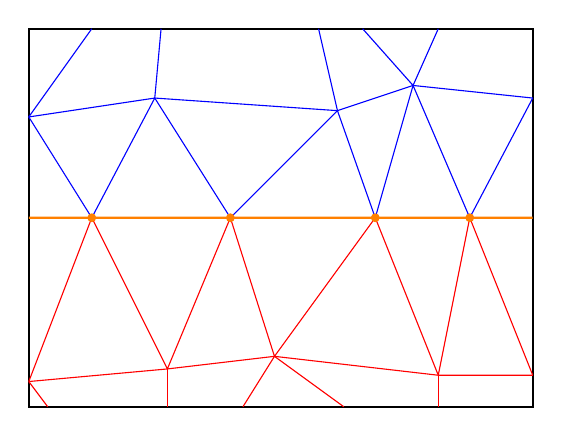
\begin{tikzpicture}[scale=0.8]
			\coordinate (a) at (1,3);
			\coordinate (b) at (3.2,3);
			\coordinate (c) at (5.5,3);
			\coordinate (d) at (7,3);
			% 
			\coordinate (aa) at (0,4.6);
			\coordinate (ab) at (2,4.9);
			\coordinate (ac) at (4.9,4.7);
			\coordinate (ad) at (6.1,5.1);
			\coordinate (ae) at (8,4.9);
			%
			\coordinate (af) at (1,6);
			\coordinate (ag) at (2.1,6);
			\coordinate (ah) at (4.6,6);
			\coordinate (ai) at (5.3,6);
			\coordinate (aj) at (6.5,6);        
			% 
			\coordinate (ba) at (0,0.4);
			\coordinate (bb) at (2.2,0.6);
			\coordinate (bc) at (3.9,0.8);
			\coordinate (bd) at (6.5,0.5);
			\coordinate (be) at (8,0.5);
			%
			\coordinate (bf) at (0.3,0);
			\coordinate (bg) at (2.2,0);
			\coordinate (bh) at (3.4,0);
			\coordinate (bi) at (5,0);
			\coordinate (bj) at (6.5,0);
			% Light grid (graph paper)
			%\draw[step=0.5cm, very thin, gray!40] (0,0) grid (8,6);
			% Slightly darker major grid every 1 cm
			%\draw[step=1cm, thin, gray!70] (0,0) grid (8,6);
			% Border of the figure
			\draw[thick] (0,0) rectangle (8,6);
			\draw[thick, orange] (0,3) -- (a) -- (b) -- (c) -- (d) -- (8, 3);
			\draw[thin, blue] (aa) -- (ab) -- (ac) -- (ad) -- (ae);
			\draw[thin, blue] (aa) -- (af);
			\draw[thin, blue] (ab) -- (ag);
			\draw[thin, blue] (ac) -- (ah);
			\draw[thin, blue] (ad) -- (ai);
			\draw[thin, blue] (ad) -- (aj);
			\draw[thin, blue] (aa) -- (a) -- (ab) -- (b) -- (ac) -- (c) -- (ad) -- (d) -- (ae);
			\draw[thin, red] (ba) -- (a) -- (bb) -- (b) -- (bc) -- (c) -- (bd) -- (d) -- (be);
			\draw[thin, red] (ba) -- (bb) -- (bc) -- (bd) -- (be);
			\draw[thin, red] (ba) -- (bf);
			\draw[thin, red] (bb) -- (bg);
			\draw[thin, red] (bc) -- (bh);
			\draw[thin, red] (bc) -- (bi);
			\draw[thin, red] (bd) -- (bj);
			\fill[orange] (a) circle (2pt);
			\fill[orange] (b) circle (2pt);
			\fill[orange] (c) circle (2pt);
			\fill[orange] (d) circle (2pt);
		\end{tikzpicture}
		\caption{First figure}
	\end{subfigure}
%	\hfill
	\begin{subfigure}{0.48\textwidth}
		\centering
		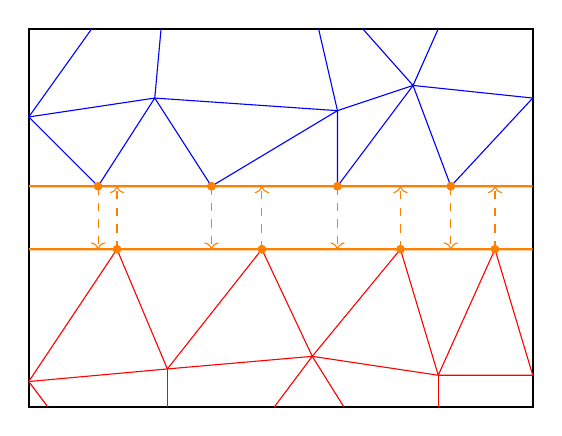
\begin{tikzpicture}[scale=0.8]
			\coordinate (a) at (1.1,3.5);
			\coordinate (b) at (2.9,3.5);
			\coordinate (c) at (4.9,3.5);
			\coordinate (d) at (6.7,3.5);
			\coordinate (as) at (1.1,2.5);
			\coordinate (bs) at (2.9,2.5);
			\coordinate (cs) at (4.9,2.5);
			\coordinate (ds) at (6.7,2.5);
			%
			\coordinate (u) at (1.4,2.5);
			\coordinate (v) at (3.7,2.5);
			\coordinate (w) at (5.9,2.5);
			\coordinate (x) at (7.4,2.5);
			\coordinate (us) at (1.4,3.5);
			\coordinate (vs) at (3.7,3.5);
			\coordinate (ws) at (5.9,3.5);
			\coordinate (xs) at (7.4,3.5);
			% 
			\coordinate (aa) at (0,4.6);
			\coordinate (ab) at (2,4.9);
			\coordinate (ac) at (4.9,4.7);
			\coordinate (ad) at (6.1,5.1);
			\coordinate (ae) at (8,4.9);
			%
			\coordinate (af) at (1,6);
			\coordinate (ag) at (2.1,6);
			\coordinate (ah) at (4.6,6);
			\coordinate (ai) at (5.3,6);
			\coordinate (aj) at (6.5,6);        
			% 
			\coordinate (ba) at (0,0.4);
			\coordinate (bb) at (2.2,0.6);
			\coordinate (bc) at (4.5,0.8);
			\coordinate (bd) at (6.5,0.5);
			\coordinate (be) at (8,0.5);
			%
			\coordinate (bf) at (0.3,0);
			\coordinate (bg) at (2.2,0);
			\coordinate (bh) at (3.9,0);
			\coordinate (bi) at (5,0);
			\coordinate (bj) at (6.5,0);
			% Light grid (graph paper)
			%\draw[step=0.5cm, very thin, gray!40] (0,0) grid (8,6);
			% Slightly darker major grid every 1 cm
			%\draw[step=1cm, thin, gray!70] (0,0) grid (8,6);
			% Border of the figure
			\draw[thick] (0,0) rectangle (8,6);
			\draw[thick, orange] (0,3.5) -- (a) -- (b) -- (c) -- (d) -- (8, 3.5);
			\draw[thick, orange] (0,2.5) -- (u) -- (v) -- (w) -- (x) -- (8, 2.5);
			\draw[thin, blue] (aa) -- (ab) -- (ac) -- (ad) -- (ae);
			\draw[thin, blue] (aa) -- (af);
			\draw[thin, blue] (ab) -- (ag);
			\draw[thin, blue] (ac) -- (ah);
			\draw[thin, blue] (ad) -- (ai);
			\draw[thin, blue] (ad) -- (aj);
			\draw[thin, blue] (aa) -- (a) -- (ab) -- (b) -- (ac) -- (c) -- (ad) -- (d) -- (ae);
			\draw[thin, red] (ba) -- (u) -- (bb) -- (v) -- (bc) -- (w) -- (bd) -- (x) -- (be);
			\draw[thin, red] (ba) -- (bb) -- (bc) -- (bd) -- (be);
			\draw[thin, red] (ba) -- (bf);
			\draw[thin, red] (bb) -- (bg);
			\draw[thin, red] (bc) -- (bh);
			\draw[thin, red] (bc) -- (bi);
			\draw[thin, red] (bd) -- (bj);
			\draw[thin, orange, dashed, ->] (a) -- (as);
			\draw[thin, orange, dashed, ->] (b) -- (bs);
			\draw[thin, orange, dashed, ->] (c) -- (cs);
			\draw[thin, orange, dashed, ->] (d) -- (ds);
			\draw[thin, orange, dashed, ->] (u) -- (us);
			\draw[thin, orange, dashed, ->] (v) -- (vs);
			\draw[thin, orange, dashed, ->] (w) -- (ws);
			\draw[thin, orange, dashed, ->] (x) -- (xs);
			\fill[orange] (a) circle (2pt);
			\fill[orange] (b) circle (2pt);
			\fill[orange] (c) circle (2pt);
			\fill[orange] (d) circle (2pt);
			\fill[orange] (u) circle (2pt);
			\fill[orange] (v) circle (2pt);
			\fill[orange] (w) circle (2pt);
			\fill[orange] (x) circle (2pt);
		\end{tikzpicture}
		\caption{Second figure}
	\end{subfigure}
	\caption{In a) the Lid-Driven Cavity setup is presented, and in b) the velocity profile obtained for the Re=100 case, compared to the points presented in REFERENCE}
	\label{fig:lid setup}
\end{figure}

When considering the numerical implementation, a renumbering of nodes was found convenient. Several matrix multiplications, and a few linear systems of equations, need to be accomplished, and the necessary matrices are smaller, and more easily assembled if the nodes are grouped. Therefore, a renumbering of nodes in the order of interface, solid phase, liquid phase vertices and liquid phase edges was done. That is, from zero to number of interface nodes, all nodes belong to the interface, and so on. The interface nodes, of course, belong both to the solid phase and fluid phase.

The final form of the linear system of equations for the fluid and solid phases is given below: \\

\[
\begin{array}{c@{\qquad}c}
	\begin{bmatrix}
		\dfrac{M}{\Delta t} + K_x & 0 & G_x \\
		0 & \dfrac{M}{\Delta t} + K_y & G_y \\
		D_x & D_y & 0
	\end{bmatrix}
	{\renewcommand{\arraystretch}{1.4}
		\begin{bmatrix}
			v_x^{n+1} \\
			v_y^{n+1} \\
			p^{n+1}
		\end{bmatrix}
	}
	=
	{\renewcommand{\arraystretch}{1.4}
		\begin{bmatrix}
			M v_x^n \\
			M v_y^n \\
			0
		\end{bmatrix}
	}
	&
	\begin{bmatrix}
		K + \dfrac{M}{\Delta t^2} & 0 \\
		0 & K + \dfrac{M}{\Delta t^2}
	\end{bmatrix}
	{\renewcommand{\arraystretch}{1.4}
		\begin{bmatrix}
			u^{n+1}_x \\
			u^{n+1}_y
		\end{bmatrix}
	}
	=
	{\renewcommand{\arraystretch}{1.4}
		\begin{bmatrix}
			\dfrac{M (2 u_x^n - u_x^{n-1})}{\Delta t^2} + f_x \\
			\dfrac{M (2 u_y^n - u_y^{n-1})}{\Delta t^2} + f_y
		\end{bmatrix}
	}
\end{array}
\] \\

The linear system of equations are solved sequentially in a staggered fashion. The fluid velocity and pressure fields are solved, and the obtained values are used to calculate the external traction acting upon the solid at the fluid-solid interface. In turn, the solid displacement is solved, and the solid velocity calculated through the following equation:

\begin{equation}
	\mathbf{v}_s^n = \frac{\mathbf{u}^n - \mathbf{u}^{n-1}}{\Delta t}
\end{equation} \\

\noindent where $\mathbf{v}_s^n$ and $\mathbf{u}_s^n$ represents the solid velocity and displacement at time $n$, $\mathbf{u}_s^{n-1}$ the displacement at time $n-1$ and $\Delta t$ the time step size.

In the next time step, when setting boundary conditions for the fluid, the solid velocity values are used at the interface nodes, in order to maintain a consistent simulation.

\section{Validation}

In order to validate the numerical solution, a series of numerical tests are presented. First, a solid beam is simulated under an uniform load to test the solid accuracy. Secondly, the fluid is tested by the classical lid driven cavity test. And finally, the interfacial forces are validated through the measurements of drag and lift coefficients of a fixed cylinder, and the movement of a spring-mounted cylinder in free flow.

\subsection{Beam}

In order to verify the solid part of the code, a test case with no fluid was executed. In Fig. \ref{fig:solid beam} a two-dimensional beam is presented. The beam of length $L=20$ is fixed at its left side, with a downwards vertical distributed load of intensity $q=1$ applied over its length. The height of the beam is $h=1$ and the elasticity modulus is $E=100000$. The displacement of the beam is easily calculated by the equation:

\begin{equation}
	u_{max} = \frac{-q L^4}{8 EI}
\end{equation} \\

\noindent where $u_{max}$, $E$, $I$ and $L$ are respectively the maximum displacement (at the right end), the elasticity modulus, the moment of inertia and the length, resulting in $u_{max}= 2.4$ for the chosen characteristics of the beam.

\begin{figure} [h]
	\centering
	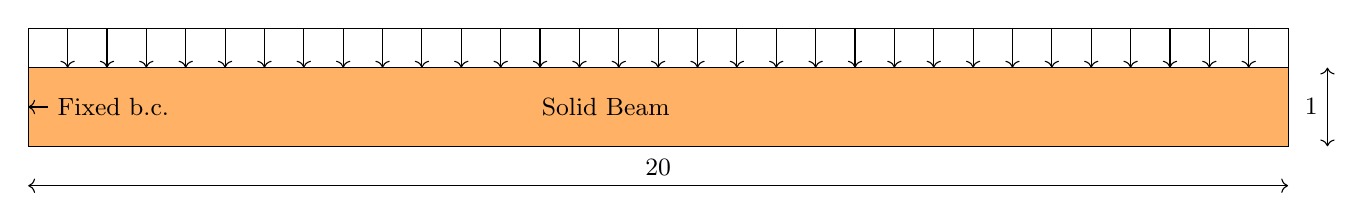
\begin{tikzpicture} [scale = 1]
		\pgfmathsetmacro\l{16}
		\pgfmathsetmacro\h{1}
		\tikzset{every node/.style={font=\small}}
		\coordinate (a) at (0,0);
		\coordinate (b) at (\l,0);
		\coordinate (c) at (\l,\h);
		\coordinate (d) at (0,\h);
		\coordinate (e) at (0,1.5*\h);
		\coordinate (f) at (\l,1.5*\h);
		\filldraw[color=orange!60] (a) -- (b) -- (c) -- (d) -- (a);
		\draw[thin, black] (a) -- (b) -- (c) -- (d) -- (a) ;
		\draw[thin, black] (d) -- (e) -- (f) -- (c);
		\draw[<->] (0, -0.5) to ["$20$"] (\l, -0.5);
		\draw[<->] (\l+0.5, 0) to ["$1$"] (\l+0.5, \h);
		\node[right] at (\l*0.4, \h/2) {Solid Beam};
		\draw[->] (+0.25,\h/2) -- +(-0.25,0);
		\node[right] at (+0.25,\h/2) {Fixed b.c.};
		\foreach \i in {1, 2, 3, 4, 5, 6, 7, 8, 9, 10, 11, 12, 13, 14, 15, 16, 17, 18, 19, 20, 21, 22, 23, 24, 25, 26, 27, 28, 29, 30, 31}
			\draw[->] (\i * 0.5, 1.5*\h) -- +(0,-\h/2);
	\end{tikzpicture}
	\caption{Solid Beam test}
	\label{fig:solid beam}
\end{figure}

The simulation was executed with a mesh of NUMBER nodes and NUMBER elements, over NUMBER times steps of $\Delta t= 0.01$ The displacement found was $u_{max numerical} = 2.399$.

\subsection{Lid-Driven Cavity Flow}

The Lid-Driven Cavity flow is a classical benchmark in the computer fluid mechanics. As seen in Fig \ref{fig:lid domain}, it consists of a cavity with no slip boundary conditions on its side and bottom walls, and an imposed horizontal velocity at the top. A point at the boundary is set to zero pressure, and the resulting velocity fields can be compared to a reference.

\pgfplotstableread[]{Files/lid_re10_vx_swapped.txt}\reavx
\pgfplotstableread[]{Files/lid_re10_vy_swapped.txt}\reavy
\pgfplotstableread[]{Files/lid_re100_vx_swapped.txt}\rebvx
\pgfplotstableread[]{Files/lid_re100_vy_swapped.txt}\rebvy
%\pgfplotstableread[]{lid_re100sl2_vx_swapped.txt}\rebslvx
%\pgfplotstableread[]{lid_re100sl2_vy_swapped.txt}\rebslvy
\pgfplotstableread[]{Files/lid_ref_re10_re100_vx.txt}\lidrefvx
\pgfplotstableread[]{Files/lid_ref_re10_re100_re400_re1000_vy.txt}\lidrefvy

\begin{figure}
\centering
\begin{subfigure}{0.47\textwidth}
	\centering
	\begin{tikzpicture} [scale=0.87]
			\begin{axis}[xlabel=$y$,
					ylabel=$v_{x}$,
					ylabel style={rotate=-90},
					xmin=0,
					xmax=1,
					ymin=-0.25,
					ymax=1,
					legend pos=north west]
					\addplot[cyan] table[x index = 0, y index=1]{\reavx};
					\addplot[orange] table[x index = 0, y index=1]{\rebvx};
					\addplot[blue, only marks, mark size=1.5pt] table[x index = 0, y index=1]{\lidrefvx};
					\addplot[red, only marks, mark size=1.5pt] table[x index = 0, y index=2]{\lidrefvx};
					\addlegendentry{Re = 10};
					\addlegendentry{Re = 100};
					\addlegendentry{Marchi 2009};
					\addlegendentry{Marchi 2009};
				\end{axis}    
		\end{tikzpicture}
	\caption{Re 10, 100, 200 e 400}
	\label{fig:lid_vx}
\end{subfigure}
\qquad
\begin{subfigure}{0.47\textwidth}
	\centering
	\begin{tikzpicture} [scale=0.87]
			\begin{axis}[xlabel=$x$,
					ylabel=$v_{y}$,
					ylabel style={rotate=-90},
					xmin=0,
					xmax=1,
					ymin=-0.3,
					ymax=0.25,
					legend pos=south west]
					\addplot[cyan] table[x index = 0, y index=1]{\reavy};
					\addplot[orange] table[x index = 0, y index=1]{\rebvy};
					\addplot[blue, only marks, mark size=1.5pt] table[x index = 0, y index=1]{\lidrefvy};
					\addplot[red, only marks, mark size=1.5pt] table[x index = 0, y index=2]{\lidrefvy};
					\addlegendentry{Re = 10};
					\addlegendentry{Re = 100};
					\addlegendentry{Marchi 2009};
					\addlegendentry{Marchi 2009};
				\end{axis}    
		\end{tikzpicture}
	\caption{Re 10, 100}
	\label{fig:lid_vy}
	\end{subfigure}
	\caption{Re 10, 100}
	\label{fig:lid}
\end{figure}

%\pgfplotstableread[]{Files/lid_re10_vy_swapped.txt}\redez
%\pgfplotstableread[]{Files/lid_re100_vy_swapped.txt}\recem
%\begin{figure}
%\centering
%\begin{subfigure}{0.48\textwidth}
%\centering
%	\begin{tikzpicture} [scale = 0.85]
%		\begin{axis}[xlabel=$t$,
%		ylabel=$v{x}$,
%		ylabel style={rotate=-90},
%		legend style={font=\footnotesize},
%		yticklabel style={/pgf/number format/fixed},
%		xmin=0,
%		xmax=1,
%		ymin=-0.4,
%		ymax=1.2,
%		ytick distance=0.1,
%		legend pos=north west]
%		\addplot[blue, thin] table[x index=0, y index=1] {\redez};
%		\addlegendentry{Numerical 48k};
%\end{axis}      
%    \end{tikzpicture}
%\caption{First- figure}
%\end{subfigure}
%\hfill
%\begin{subfigure}{0.48\textwidth}
%\centering
%	\begin{tikzpicture} [scale = 0.85]
%    		\begin{axis}[xlabel=$t$,
%		    	ylabel=$v{x}$,
%		    	ylabel style={rotate=-90},
%		    	legend style={font=\footnotesize},
%		    	yticklabel style={/pgf/number format/fixed},
%		    	xmin=0,
%		    	xmax=1,
%		    	ymin=-0.39,
%		    	ymax=1.2,
%		    	ytick distance=0.1,
%		    	legend pos=north west]
%		    	\addplot[blue, thin] table[x index=0, y index=1] {\recem};
%		    	\addlegendentry{Numerical 48k};
%		    \end{axis}      
%    \end{tikzpicture}
%\caption{Second figure}
%\end{subfigure}
%\caption{In a) the Lid-Driven Cavity setup is presented, and in b) the velocity profile obtained for the Re=100 case, compared to the points presented in REFERENCE}
%\label{fig:lid setup}
%\end{figure}

The simulations were executed with NUMBER elements, with a time step equal to NUMBER, over Reynolds numbers $Re=10$, $Re=100$, $Re=1000$. The results obtained are displayed in Fig \ref{tab:lid setup}.

\subsection{Drag and Lift Coefficients}

To validate the forces acting upon the solid walls calculated by the numerical simulation, the drag and lift coefficients obtained over the simulation of a fixed cylinder inside a fluid domain over several Reynolds numbers were measured and compared to available references in the literature, such as the works of  REF REF REF. The simulation domain used is presented in Fig \ref{fig:drag domain}

\begin{figure} [h]
	\centering
	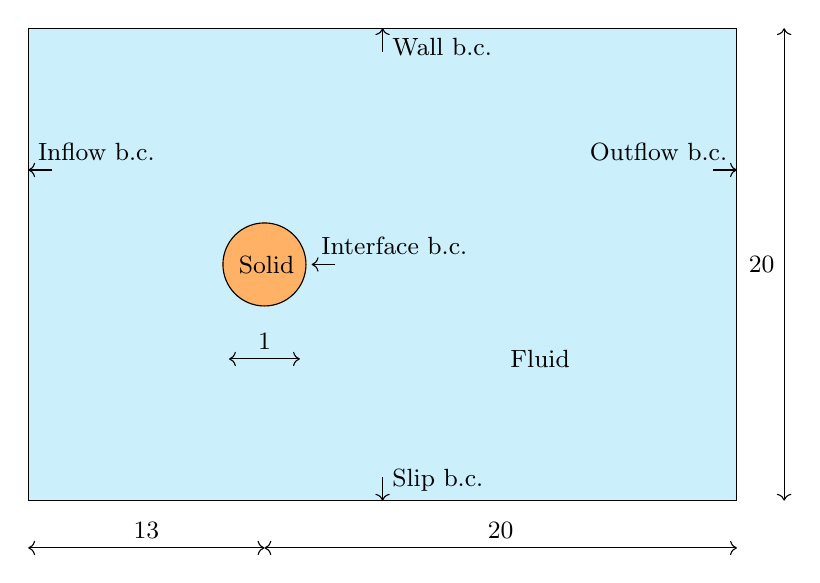
\begin{tikzpicture} [scale = 3]
		\pgfmathsetmacro\f{1}
		\tikzset{every node/.style={font=\small}}
		\coordinate (a) at (0,0);
		\coordinate (b) at (3,0);
		\coordinate (c) at (3,2);
		\coordinate (d) at (0,2);
		\filldraw[color=cyan!20] (a) -- (b) -- (c) -- (d) -- (a) ;
		\draw[thin, black] (a) -- (b) -- (c) -- (d) -- (a) ;
		\filldraw[color=orange!60] (1,1) circle (5pt);
		\draw[thin, black] (1,1) circle (5pt);
		\draw[<->] (0, -0.2) to ["$13$"] (1, -0.2);
		\draw[<->] (1, -0.2) to ["$20$"] (3, -0.2);
		\draw[<->] (3.2, 0) to ["$20$"] (3.2, 2);
		\draw[<->] (0.85, 0.6) to ["$1$"] (1.15, 0.6);
		\draw[->] (1.5,0.1) -- +(0,-0.1) node[above right] {Slip b.c.};
		\draw[->] (0.1,1.4) -- +(-0.1,0) node[above right] {Inflow b.c.};
		\draw[->] (2.9,1.4) -- +(0.1,0) node[above left] {Outflow b.c.};
		\draw[->] (1.5,1.9) -- +(0,0.1) node[below right] {Wall b.c.};
		\draw[->] (1.3,1) -- +(-0.1,0) node[above right] {Interface b.c.};
		\node[right] at (2, 0.6) {Fluid};
		\node[right] at (0.85, 1) {Solid};
	\end{tikzpicture}
	\caption{Drag Coefficient Test Domain}
	\label{fig:drag domain}
\end{figure}

The drag and lift coefficients obtained in the simulations over several Reynolds numbers can be compared to the references in Fig. \ref{fig:drag coeff}. Good agreement with the different references can be observed.

\pgfplotstableread[]{Files/placzek_12k_a_28-Jan_drag_out.txt}\drag
\pgfplotstableread[]{Files/placzek_12k_a_28-Jan_lift_out.txt}\lift
\begin{figure}
\centering
\begin{subfigure}{0.45\textwidth}
\centering
\begin{tikzpicture}
		\begin{axis}[xlabel=$t$,
			ylabel=$C_{D}$,
			ylabel style={rotate=-90},
			legend style={font=\footnotesize},
			yticklabel style={/pgf/number format/fixed},
			xmin=0,
			xmax=150,
			ymin=1,
			ymax=1.6,
			ytick distance=0.1,
			legend pos=south east]
			%			\addplot[orange] table[x index = 0, y index=1]{\rebvx};
			%\addplot[red, thin] {1.5*(1 - ((2*\x - 1)*(2*\x - 1)))};
			\addplot[blue, thin] table[x index=0, y expr=\thisrowno{1}/500] {\drag};
			%\addplot[purple, only marks, mark size=1pt] table[x index = 0, y index=1]{\refs};
			%			\addplot[red, only marks, mark size=1.5pt] table[x index = 0, y index=2]{\lidrefvx};
			\addlegendentry{Numerical 48k};
		\end{axis}  
        \end{tikzpicture}
\caption{Drag coefficient}
\end{subfigure}
\hfill
\begin{subfigure}{0.45\textwidth}
\centering

\begin{tikzpicture}
	\begin{axis}[xlabel=$t$,
		ylabel=$C_{L}$,
		ylabel style={rotate=-90},
		legend style={font=\footnotesize},
		yticklabel style={/pgf/number format/fixed},
		xmin=0,
		xmax=150,
		ymin=-0.4,
		ymax=0.4,
		ytick distance=0.1,
		legend pos=south west]
		%			\addplot[orange] table[x index = 0, y index=1]{\rebvx};
		%\addplot[red, thin] {1.5*(1 - ((2*\x - 1)*(2*\x - 1)))};
		\addplot[blue, thin] table[x index=0, y expr=\thisrowno{1}/500] {\lift};
		%\addplot[purple, only marks, mark size=1pt] table[x index = 0, y index=1]{\refs};
		%			\addplot[red, only marks, mark size=1.5pt] table[x index = 0, y index=2]{\lidrefvx};
		\addlegendentry{Numerical 48k};
	\end{axis} 
\end{tikzpicture}
\caption{Lift}
\end{subfigure}
\caption{}
\label{fig:drag lift results}
\end{figure}

% \begin{figure}
% 	\begin{tikzpicture}
% 		\begin{axis}[
% 			xlabel={$Re$},
% 			ylabel={$C_D$},
% %			grid=major,
% 			legend pos=north east,
% 			enlargelimits=0.1
% 			]
			
% 			% Reference data
% 			\addplot[only marks, color=red, mark=*] coordinates {
% 				(10, 2.5)
% 				(20, 1.8)
% 				(30, 1.5)
% 				(40, 1.3)
% 			};
% 			\addlegendentry{Reference}
			
% 			% Your data
% 			\addplot[only marks, color=blue, mark=square*] coordinates {
% 				(10, 2.4)
% 				(20, 1.7)
% 				(30, 1.4)
% 				(40, 1.2)
% 			};
% 			\addlegendentry{Your Data}
			
% 		\end{axis}
% 	\end{tikzpicture}	
% \end{figure}

\subsection{Spring Mounted Cylinder}

The final test for the fluid forces acting upon the cylinder is the measure of the amplitude of movement for a spring-mounted cylinder in free flow. This cylinder is fixed in the $x$ direction, and attached to a spring on the $y$ direction, that resists it movement. The spring has an effective stiffness presented in \ref{shiels} given by:

\begin{equation}
    k_{eff} = 
\end{equation}

\section{Results}

\begin{figure}
	\centering
	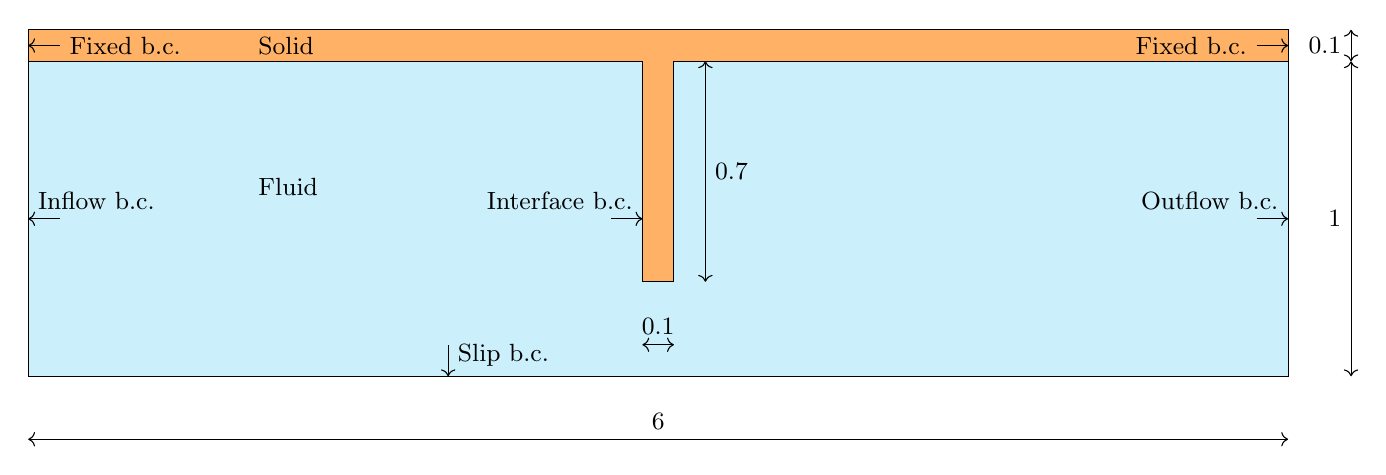
\begin{tikzpicture} [scale = 4]
		\pgfmathsetmacro\l{4}
		\pgfmathsetmacro\h{1}
		\pgfmathsetmacro\w{0.1}
		\pgfmathsetmacro\s{0.7}
		\tikzset{every node/.style={font=\small}}
		\coordinate (a) at (0,0);
		\coordinate (b) at (\l,0);
		\coordinate (c) at (\l,\h);
		\coordinate (d) at (0,\h);
		\coordinate (e) at (\l/2-\w/2,\h);
		\coordinate (f) at (\l/2-\w/2,\h-\s);
		\coordinate (g) at (\l/2+\w/2,\h-\s);
		\coordinate (h) at (\l/2+\w/2,\h);
		\coordinate (i) at (0,\h+\w);
		\coordinate (j) at (\l,\h+\w);		
		\filldraw[color=cyan!20] (a) -- (b) -- (c) -- (d) -- (a);
		\filldraw[color=orange!60] (e) -- (f) -- (g) -- (h) -- (d) -- (i) -- (j) -- (c) -- (e);
		\draw[thin, black] (d) -- (a) -- (b) -- (c) -- (h) -- (g) -- (f) -- (e) -- (d) -- (i) -- (j) -- (c);
		\draw[<->] (0, -0.2) to ["$6$"] (\l, -0.2);
		\draw[<->] (\l+0.2, 0) to ["$1$"] (\l+0.2, \h);
		\draw[<->] (\l+0.2, \h) to ["$0.1$"] (\l+0.2, \h +\w);
		\draw[<->] (\l/2-\w/2, 0.1*\h) to ["$0.1$"] (\l/2+\w/2, 0.1*\h);
		\draw[<->] (\l/2+\w/2+0.1, \h) to ["$0.7$"] ( \l/2+\w/2+0.1, \h-\s);
		\draw[->] (\l/3,0.1) -- +(0,-0.1) node[above right] {Slip b.c.};
		\draw[->] (0.1,\h/2) -- +(-0.1,0) node[above right] {Inflow b.c.};
		\draw[->] (\l-0.1,\h/2) -- +(0.1,0) node[above left] {Outflow b.c.};
		\draw[->] (\l/2 -\w/2 -0.1,\h/2) -- +(0.1,0) node[above left] {Interface b.c.};
		\draw[->] (+0.1,\h + 0.05) -- +(-0.1,0);
		\draw[->] (\l -0.1,\h + 0.05) -- +(0.1,0);
		\node[right] at (+0.1,\h + 0.05) {Fixed b.c.};
		\node[left] at (\l-0.1,\h + 0.05) {Fixed b.c.};
		\node[right] at (0.7, 0.6) {Fluid};
		\node[right] at (0.7, 1.05) {Solid};
	\end{tikzpicture}
	\caption{Test Domain}
	\label{fig:2d static/osc setup}
\end{figure}

\section{Conclusion}

\section{Declaration of Interests}

The authors declare that they have no known competing financial interests or personal relationships that could have appeared to influence the work reported in this paper.

\section{CRediT authorship contribution statement}

\textbf{Daniel B. V. Santos:} Methodology, Software, investigation, Writing - Original Draft, Writing - Review \& Editing.

\textbf{Gustavo R. Anjos:} Methodology, Resources, Writing - Review \& Editing, Supervision.

\textbf{Marcelo A. Savi:} Conceptualization, Writing - Review \& Editing, Supervision, Funding Acquisition. 

\section{Acknowledgements}



\bibliographystyle{alpha}
\bibliography{sample}

\end{document}